\documentclass[a4paper,12pt]{article}

\usepackage[a4paper, inner=1.7cm, outer=2.7cm, top=1.5cm, bottom=2cm, bindingoffset=1.2cm]{geometry}
\usepackage[german]{babel}
\usepackage{microtype}
\usepackage{fancyhdr}
\usepackage{hyperref}
\usepackage[pdftex]{graphicx}

\pagestyle{fancy}
\fancyfoot[C]{\thepage}

\newcommand{\myparagraph}[1]{\paragraph*{#1}\mbox{}\\}

\title{Dokumentation zur Projektaufgabe für das Modul Künstliche Intelligenz für Spiele im Wintersemester 2022/23} 
\author{Oliver Jakobs}

\begin{document}

\maketitle

\section*{Thema und Motivation}

Als Thema für meine Modulaufgabe habe ich mich für \textbf{Decision Trees} entschieden. 

Einlesen eines Decision Trees aus einer XML-Datei und Frage-Antwort Spiel oder textbasiertes Adventure.

Das Konzept lässt sich neben künstlicher Intelligenz auch auf viele andere Bereiche anwenden. Ein Beispiel ist eine Alternative zu Zustandsautomaten um festzulegen welche Animation gespilet werden soll.

\newpage

\section*{Allgemeine Designentscheidungen}

Mein Programm lässt sich in zwei Abschnitte aufteilen. Der erste Teil ist die Implementiation des Decision Tress. Dieser wird aus einer .xml-Datei eingelesen und in eine passenden Datenstruktur geladen. 
Den zweiten Teil habe ich TreeWalker gennant. Dieser Teil beschäftigt sich mit Kommunikation zwischen dem Nutzer und dem Baum. 
\\
\\
Das Programm habe ich bewusst im C-Style programmiert. Das heißt ich habe mich bei der Struktur des Programmes an C gehalten und habe lediglich einzelene Features (z.B. \texttt{std::vector} oder \texttt{std::variant}) aus C++ verwendet.
Der Grund für diese Entscheidung war, dass ich privat hauptsächlich in C programmiere und so am komfortabelsten mit diesem Stil bin. Außerdem habe ich so weniger Aufwand, wenn ich die Implementation anpassen muss, wenn ich Decision Trees in meinen C-Programmen verwenden will.
\\
\\
Um ein Beispiel zu haben, mit dem ich mein Programm testen kann habe ich online nach einfachen Entscheidungsbäumen gesucht und hier (\url{https://heartbeat.comet.ml/understanding-the-mathematics-behind-decision-trees-22d86d55906}) einen gefunden, mit dem ich (fast) alle geplanten Features demonstrieren kann. 

\begin{figure}[h]
	\centering
	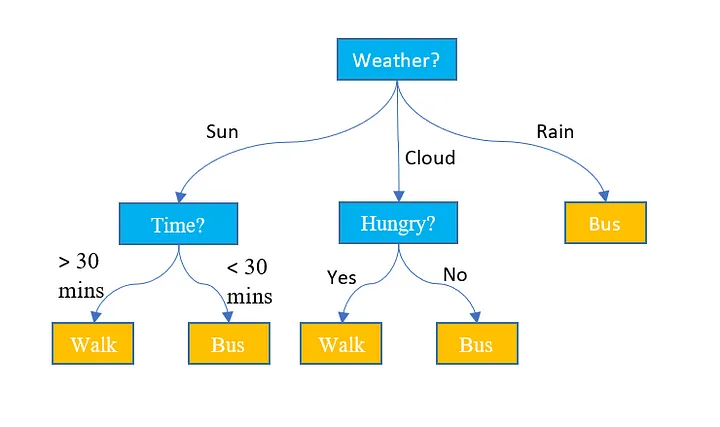
\includegraphics[width=\linewidth]{tree.png}
\end{figure}

Zwei Features haben mir noch gefehlt, aber diese konnte ich mit kleinen Anpassungen (ohne dabei die Ergebnisse zu verändern) auch noch darstellen.
Mit diesem Baum habe ich dann meine XML-Struktur definiert und danach mein Programm implementiert. 

\newpage
\section*{Entscheidungen zur XML-Datei}
In der XML-Datei kann neben dem Entscheidungsbaum auch noch Zusatzinformationen angegeben werden, um die Interaktion mit dem Entscheidungsbaum zu vereinfachen. 
Das Root-Element der XML-Datei habe ich \texttt{decisiontree}. Aber da ich dafür keine Abfrage implementiert habe, kann man das im Grunde so nennen wie man möchte.

\myparagraph{Zusatzinformationen}
Mit dem Tag \texttt{intro} kann ein Einleitungstext angegeben werden. 
Mit dem Tag \texttt{prompt} kann definiert werden welche Frage der TreeWalker für eine Entscheidung stellen soll.
Und mit dem Tag \texttt{result} können Beschreibungen der Ergebnisse angegeben werden. Hier muss dann noch der Name des Ergebnisses als Attribut angegeben werden.

\myparagraph{Entscheidungsbaum}
Der eigentliche Entscheidungsbaum besteht aus vier Tags (\texttt{decision}, \texttt{option}, \texttt{final} und \texttt{invalid}). 
Diese Tags entsprechen dem Type der TreeNodes, die aus diesem Element generiert werden.
Außerdem können Elemente mit diesen Tags noch einen Namen (\texttt{name}) und einen Wert (\texttt{value}) als Attribut haben.

\myparagraph{Beispiel}
Wi oben erwähnt muss der Beispielsbaum noch bisschen angepasst werden. 
Die erste Anpassung nutzt den \texttt{invalid} Tag um bei der Entscheidung \emph{Time?} negative Antworten zu verhindern.
Die zweite Anpassung habe ich letztendlich nur gemacht um ein Interval als Antowrtmöglichkeit angeben zu können.
Wenn man dann den angepassten Baum dann mit meiner XML-Struktur darstellt, kann das wie folgt aussehen:

\begin{verbatim}
<decisiontree>
  <intro>Deciding whether to walk or take the bus.</intro>
  <option name="weather">
    <prompt>How is the weather? (sunny/cloudy/rain)</prompt>
    <decision value="sunny" name="time">
      <prompt>How much time do you have (in minutes)?</prompt>
      <invalid value="&lt;0"/>
      <final value="0:29" name="walk" />
      <final value="&gt;=30" name="bus" />
    </decision>
    <option value="cloudy" name="hungry">
      <prompt>Are you hungry? (yes/no)</prompt>
      <final value="yes" name="walk" />
      <final value="no" name="bus" />
    </option>
    <final value="rain" name="bus" />
  </option>

  <result name="walk">You should walk.</result>
  <result name="bus">You should take the bus.</result>
</decisiontree>
\end{verbatim}

\newpage
\section*{Entscheidungen zur DecisionTree Implementation}
Der DecisionTree wird aus mehreren TreeNodes aufgebaut. So eine TreeNode hat einen Type, einen Namen, einen Wert und eine Liste an Nachfolgern. Anhand der Types werden folgende Arten von TreeNodes unterschieden:

\myparagraph{Decision}
TreeNodes mit dem Type \texttt{decision} bilden den Grundbaustein meiner Implementation. An sich lässt sich alle Funktionalität von DecisionTrees nur mit TreeNodes dieser Art umsetzen.

Der Wert einer \texttt{decision} ist eine Boolean Expression, in die zum Zeitpunkt der Entscheidung eine Variable eingesetzt werden kann. Operatoren in diesen Expressions sind die Standartoperatoren ($<, <=, >, >=$) und ein Intervall Operator (angegeben mit $v_1:v_2$). Gibt die Expression \texttt{True} zurück, so ist die entsprechende TreeNode die richtige Antwort.

In meiner Implementation sind alle numerischen Werte \texttt{Integers}, da \texttt{Float}-Werte den Umfang und den damit verbundenen Aufwand sehr stark in die Höhe treiben würden.
Außerdem ist die Umsetzung von Float-Werten (bis auf das Erkennen und Parsen) gleich mit der Umsetzung der Integer-Werte und bringt daher keine neuen Herausforderungen. 

\myparagraph{Option}
Bei einer TreeNode mit dem Type \texttt{option} können die Antwortmöglichkeiten als Zeichenketten angegeben werden. Die gegebene Antwort wird mit allen diesen Zeichenketten (mit \texttt{std::string::compare}) verglichen und die erste passende Option wird ausgewählt.

\myparagraph{Final}
Eine TreeNode ist \texttt{final}, wenn sie keine Nachfolger hat (also ein Blatt ist). In der XML-Datei kann der entsprechende Tag verwendet werden, um das zu verdeutlichen.

\myparagraph{Invalid}
Mit einer \texttt{invalid} TreeNode können bestimmte Werte blockiert werden. So können zum Beispiel alle Werte $<0$ als ungültige Antwort makiert werden.
\\
\\
Wenn über einen Knoten im Baum entschieden wird, wird jeder Nachfolger nacheinander angeschaut. Dabei wird der erste Treffer wird akzeptiert. Die Antwort ist ungültig, wenn kein passender Knoten gefunden wurde, wenn die Eingabe das falsche Format hat (z.B. kein \texttt{int}-Wert als Eingabe für eine \texttt{decision}) oder wenn der (erste) gefundene Knoten \texttt{invalid} ist. 

\newpage
\section*{Bedienung}

Um das Programm zu starten muss die Datei \texttt{DecisionTree.exe} ausgeführt werden. Dafür wird neben der \texttt{.exe} auch der Ordern \texttt{./res/} mit Inhalt benötigt.
Beim Starten über die Kommandozeile kann noch ein Pfad zu einer XML-Datei als Argument angegeben werden, um einen eigenen Entscheidungsbaum zu laden. 
\[\texttt{.\textbackslash DecisionTree.exe [filename]}\]
Wird kein Argument angegeben wird der oben vorgestellte Beispielsbaum als Default geladen.
\\
\\
Die Ausführung des Programms findet in einem \texttt{read-eval-print loop (REPL)} statt. Dem Nutzer wird eine Frage gestellt, auf die er dann antworten muss. Ist die Antwort ungültig, das heißt die Antwort entspricht nicht der erwarteten Form oder ist keine der möglichen Antwortmöglichkeiten, so wird der Nutzer erneut aufgefordert zu antworten. 
Wenn ein Blatt des Entscheidungsbaumes erreicht wird, wird das Endergebnis angezeigt und das Programm beendet.

\section*{Bibliotheken}

Da dieses Projekt textbasiert ist benötige ich nur eine Möglichkeit XML-Dateien einzulesen. Für diese Funktionalität habe ich mich für die Bibliothek \textbf{TinyXML-2} (\url{https://github.com/leethomason/tinyxml2}) entschieden.
Die Bibliothek besteht aus zwei Dateien (einer \texttt{.h} und einer \texttt{.cpp}), die ich einfach in mein Projekt eingefügt habe.

\section*{Build}

Zur Project Generation benutze ich Premake (\url{https://premake.github.io/}). Ich habe die entsprechenden Scripts meiner Abgabe beigefügt.
Falls also Probleme mit der VisualStudio Solution autreten sollten,
kann mit dem folgenden Befehl das Projekt neu generiert werden und so die Probleme hoffentlich gelöst werden:
\[\texttt{.\textbackslash premake\textbackslash premake5.exe [action]}\]
Für mein Projekt habe ich \texttt{vs2019} als \texttt{action} verwendet. Andere Möglichkeiten sind hier \url{https://premake.github.io/docs/Using-Premake} aufgelistet.


\end{document}